\section{Qualitätsmanagement und Qualitätssicherung}
\label{sec:qualitaetsmanagement}
Die Software ist ein großer Teil unseres Lebens geworden und ist Bestandteil vieler Produkte, die wir nutzen: von den Handys bis zu den Autos. 
Wir erwarten, dass die Programme korrekt und fehlerlos funktionieren, ohne dabei nachzudenken, welcher Verwaltung- und Sicherungsaufwand dahintersteckt. 
Wenn diese Anforderungen erfüllt werden, spricht man von „guter Qualität“. \cite[1,2]{Schn:2012:Abenteuer:} Was bedeutet überhaupt \glqq gute Qualität\grqq{} und wie lässt sich diese messen?
Welche Maßnahmen sind dabei notwendig, um die hohe Qualität zu leisten? Welche Ansätze zur Qualitätssicherung sind für welche Projektgrößen und Vorgehensmodellen anwendbar und besonders vorteilhaft? 
In diesem Kapitel wird versucht, diese Fragen zu beantworten.

\subsection{Definition und Eingrenzung}
\label{subsec:qualitaetsmanagement:eingrenzung}
Es gibt unterschiedliche Wege, die Softwarequalität zu bewerten. In der Softwareentwicklung wird häufig der Standard ISO/IEC 9126 zur Bewertung der Softwarequalität verwendet. 
Diese Norm definiert den Begriff Software-Qualität als: 
\begin{quote}
    \glqq Gesamtheit der Merkmale und Merkmalswerte eines Software-Produkts, die sich auf dessen Eignung beziehen, festgelegte Erfordernisse zu erfüllen.\grqq{} \cite[6]{Hoff:2008:Software:}
\end{quote}
Konkret bedeutet das, dass die Software-Qualität sich aus mehreren verschiedenen Kriterien zusammensetzt. 
Der Standard definiert dabei 6 Qualitätsmerkmale: Funktionalität, Zuverlässigkeit, Benutzbarkeit, Effizienz, Wartbarkeit und Portierbarkeit. 
Dabei beeinflussen sich die Merkmale gegenseitig: positiv und negativ. Zum Beispiel, eine Verbesserung der Wartbarkeit ergibt eine Verbesserung der Funktionalität, aber eine Verschlechterung der Effizienz. 
Somit lässt sich sagen, dass eine Verbesserung aller Qualitätsmerkmale gleichzeitig nicht möglich und ein Kompromiss zu suchen ist \cite[11]{Hoff:2008:Software:}\cite[132]{Goll:2011:Methoden:}. 
Um die Software-Qualität optimal zu verbessern, werden Maßnahmen zur Qualitätssicherung gebraucht. Diese lassen sich in die Produktqualität- und Prozessqualitätsmaßnahmen unterteilen. 
\\Bei der Produktqualität steht das Softwareprodukt im Vordergrund. Die Maßnahmen dieser Gruppe werden in konstruktive Maßnahmen (Fehlervermeidung während der Entwicklung) und analytische Maßnahmen (Fehlerfindung nach der Entwicklung) unterteilt. 
\\Die Prozessqualität umfasst die in Kapitel \ref{sec:zusammenarbeit} beschriebenen Vorgehensmodellen und andere Verwaltungstechnologien. Für diese Arbeit wird der Bereich der Prozessqualität. Es werden lediglich
die Auswirkungen und Vorteile auf die Projekte in unterschiedlichen Vorgehensmodellen beim Einsatz der verschiedenen Produktqualitätsmaßnahmen beschrieben. 

\subsection{Konstruktive Qualitätssicherung}
\label{subsec:qualitaetsmanagement:konstruktive}
Zu dem Gebiet der konstruktive Qualitätssicherung fallen insbesondere Maßnahmen, die eine frühzeitige Erkennung und Vermeidung der Fehler während des Entwicklungsprozesses ermöglichen. In diesem Kapitel werden 3 wichtigsten davon: 
\textbf{Softwarerichtlinien}, \textbf{Vertragsbasierte} Programmierung und \textbf{Dokumentation} vorgestellt.  
\\\textbf{Softwarerichtlinien} bezeichnen alle Mittel, die den Programmierprozess über die syntaktischen und semantischen Regeln der jeweiligen Programmiersprache hinweg regelt \cite[65]{Hoff:2008:Software:}. 
Die wichtigsten Ziele dieser Maßnahmen sind \textit{Vereinheitlichung} und \textit{Fehlerreduktion}. Um diese Ziele zu erreichen, werden \textit{Notations-} und \textit{Sprachkonventionen} eingesetzt.  
\\

Die meisten Software-Ingenieure entwickeln im Laufe der Jahre ihren eigenen Programmier-Stil, worauf sich die Person gewohnt. In Teams kann diese Tatsache aber dazu führen, dass mehrere Mitarbeiter den Code von anderen nicht richtig verstehen oder mehr Zeit dafür brauchen. 
Um dieses Problem zu lösen, werden \textbf{Notationskonventionen} verwendet. Diese umfassen die Namensgebung der verwendeten Strukturen und Variablen, die Verwendung von Leerzeilen und Charakteristik und die Dokumentation des geschriebenen Codes. 
Oft gibt es unternehmensspezifische Konventionen, dennoch haben sich folgende Notationsvorschriften in der Software-entwicklung durchgesetzt:
\begin{itemize}
    \item \textbf{Pascal Case}: die Variablennamen beginnen mit dem Großbuchstaben und jedes weitere Wort wird ohne Trennzeichen mit großen Buchstaben eingefügt (z.B. ForegroundColor). 
    \item \textbf{Camel Case}: gleich wie Pascal Case, aber das erste Wort wird mit Kleinbuchstaben angefangen (foregroundColor).
    \item \textbf{Uppercase/Lowercase}: der gesamte Name wird entweder in Groß- oder Kleinbuchstaben geschrieben (FOREGROUNDCOLOR).
\end{itemize}
Oft werden verschiedene Notationsstile miteinander kombiniert, damit verschiedene Arten von Bezeichner dargestellt werden. Dies sorgt für ein besser lesbares und verständliches Code. 
\\Um ein weiteres Ziel der Softwarerichtlinien, die Fehlerreduktion, zu ermöglichen, werden die \textbf{Sprachkonventionen} verwendet. 
Im Gegensatz zu den Notationskonventionen, werden hier die Entwickler darin eingeschränkt, bestimmte Sprach-Konstrukte unter bestimmten Voraussetzungen zu verwenden. Dazu gehören zum Beispiel, mit welchen Variablentypen auf die einzelnen Bits zugegriffen werden darf (unsigned int in MISRA C Standard) \cite[76]{Hoff:2008:Software:} \cite{Misr:02122022:MISRA:}.   
\\

Einen weiteren Bestandteil der konstruktiven Qualitätssicherung bildet die \textbf{Vertragsbasierte} Programmierung. Das Konzept wurde von Bertrand Meyer unter dem Namen Design by contract eingeführt \cite{Meye:1992:Applying:1}. 
Kurz beschrieben, basiert die vertragsbasierte Programmierung auf den folgenden Prinzipien:
\begin{itemize}
    \item \textbf{Vor- und Nachbedingungen}: die Objekte müssen bestimmte Voraussetzungen erfüllen, um Routinen betreten und verlassen zu können. Dafür werden bestimmte „require“ Blöcke in das Programm eingefügt.
    \item \textbf{Invarianten}: im Programm werden globale Beschränkungen der Wertebereiche bestimmter Variablen und Strukturen gesetzt.
    \item \textbf{Zusicherungen}: bezeichnen die Überprüfungen, die im Gegensatz zu Invarianten nur an der Stelle des Auftretens ausgewertet werden.
\end{itemize}  
All diese Prinzipien werden auch heute bei der Anforderungsspezifikation und für die Definition von Tests eingesetzt \cite[96]{Hoff:2008:Software:} \cite{Meye:1992:Applying:1}
\\

Verwaltung der \textbf{Projektdokumentation} ist auch eine wichtige Maßnahme zur Herstellung der Qualitätssicherheit. Dabei lässt sich diese in die externen und internen Dokumente aufteilen. 
Die externe Dokumentation dient dem Austausch mit dem Kunden. Diese hat oft, insbesondere in großen Projekten klare Vorgaben und Muster wie sie zu erstellen ist (z.B. für Pflichtenheft) \cite[141]{Hoff:2008:Software:}. 
Bei der internen Dokumentation handelt es sich um andere Dokumente, die nur unternehmensintern zur Verfügung stehen. Diese Dokumente umfassen zum einen die oben beschriebene Software-Richtlinien und auch die Programmdokumentation und andere Spezifikationen. 
\\Einer der wichtigsten Dokumente in vielen Vorgehensmodellen ist die Spezifikation. In dem Dokument werden die Anforderungen an ein Software-System genauer beschrieben. 
Diese Spezifikation kommt daher oft als externes Dokument und wird bei vielen Projekten formal gehalten. Die Anwender tauschen dann während der Entwicklung die sogenannten Implementierungsdokumente aus, wo anhand von Kommentaren im Code die implementierten Funktionen beschrieben werden. 
Die Formulierung dieser Dokumente kann großen Aufwand, vor allem in dokumenten-basierten Vorgehensmodellen beanspruchen, weswegen auch viele dieser Modelle, wie z.B. das V-Modell kritisiert wird. \cite{IJC:2015:Related:} 
\subsection{Analytische Qualitätssicherung}
\label{subsection:qualitaetsmanagement:analytische}
Bei der analytischen Qualitätssicherung wird, im Gegensatz zur konstruktiven, geht es nicht um Fehlervermeidung, sondern um Fehlerfindung und Beseitigung nach dem Entwicklungsprozess \cite[20]{Hoff:2008:Software:} \cite[132]{Goll:2011:Methoden:}. 
Dies wird mithilfe verschiedener Test- und Verifikationsverfahren nach und während der Entwicklung ermöglicht. Diese werden im Folgenden vorgestellt. 
\subsubsection{Software-Tests}
\label{subsubsec:qualitaetsmanagement:tests}
Bereits im Jahr 1979 war in der Software-Entwicklung bekannt, dass ungefähr die Hälfte der Zeit- und Geldkosten in das Testen investiert werden muss \cite{Myer:2012:art:}. 
Diese Tatsache hat sich bis heute nicht wesentlich verändert, wenn überhaupt, nimmt die Implementierung und Durchführung der Tests in manchen Projekten einen wesentlich höheren Anteil an Aufwand. 
Diese Tests lassen sich bezüglich verschiedener Merkmale in verschiedene Klassen einteilen \cite[158]{Hoff:2008:Software:}: 
\begin{itemize}
    \item \textbf{Prüfebene}: In welcher Projektphase wird der Test durchgeführt?
    \item \textbf{Prüfkriterium}: Welche inhaltlichen Aspekte werden getestet?
    \item \textbf{Prüfmethodik}: Wie werden die Tests konstruiert?
\end{itemize}
In dieser Arbeit werden verschiedene Testarten anhand ihres Prüfkriteriums vorgestellt. Diese Tests werden anhand ihres Inhaltes unterschieden und können dabei in 3 Kategorien unterteilt werden: Funktionale, Operationale und Temporale Tests.
Die wichtigsten Arten von \textbf{funktionalen} Tests sind \cite[170]{Hoff:2008:Software:} \cite[242]{Meye:2018:Softwareentwicklung:}:
\begin{itemize}
    \item \textbf{Funktionstests}: sind die am häufigsten verwendete Tests, bei diesen Tests wird überprüft, ob ein richtiges Ergebnis geliefert wurde, also ob die Applikation korrekt läuft.
    \item \textbf{Crashtests}: es wird versucht, ein System zum Abstürzen zu kriegen. Es findet eine gezielte Suche nach Schwachstellen statt, durch die Bekämpfung dieser, können sicherheitskritische Systeme geschützt werden.
    \item \textbf{Zufallstests}: es wird nicht mit vorgegebenen, gezielt erzeugten Eingabedaten getestet werden, sondern mit zufälligen. Da diese Methode aber schwer systematisch anzuwenden ist, kann sie nur als Ergänzung verwendet werden.    
\end{itemize}
Die \textbf{operationalen} Tests beinhalten im Großen und Ganzen die Installation, Sicherheit und Bedienbarkeit von Systemen. Diese Tests sind insbesondere in der Web-Branche und anderen modernen Applikation wichtig, da die Bedienbarkeit und User-Experience häufig im Vordergrund stehen \cite[170-174]{Hoff:2008:Software:} \cite[242]{Meye:2018:Softwareentwicklung:}.
In den \textbf{temporalen} Tests werden vor allem die Effizienz und Schnelligkeit von Software getestet. Zum Beispiel wird es bei \textit{Last-} und \textit{Stresstesten} geprüft, wie sich ein System an den oder über den definierten Grenzen verhält. 
Die Geschwindigkeit von Software wird in den \textit{Komplexitäts-} und \textit{Laufzeittests} ermittelt, wodurch auch entschieden werden kann, ob die implementierten Algorithmen den Anforderungen entsprechen. 
\subsubsection{Statische Analyze und Verifikation}
\label{subsubsec:qualitaetsmanagement:statAnalyze}
Durch die \textbf{statische Code-Analyze} umfasst alle Maßnahmen, bei denen der Quellcode ohne Programmausführung untersucht wird. Die untersuchenden Bestandteile des Codes werden mithilfe von Software-Metriken beschrieben. 
Durch diese Analyze wird die Zuverlässigkeit und die Funktionalität des Codes geprüft. Zu den verbreiteten Software-Metriken gehören die LOC (Lines of Code) und NCSS (Non-Commented Source Statements). Bei diesen Software-Metriken wird die Anzahl der geschriebenen
Programmzeilen, bzw. ausführbaren Zeilen des Codes gezählt und dadurch wird eine grobe Aussage über die Programmkomplexität gemacht \cite[249,250]{Hoff:2008:Software:}. Jedoch sagt dieser Ansatz in der Realität nicht viel über das Programm aus, weil unterschiedliche Programmiersprachen
unterschiedliche Anzahlen von Befehlen und dadurch Zeilen haben können und auch den Aspekt der optimalen Nutzung der Werkzeuge betrachtet werden muss. Deswegen werden heutzutage viele andere Metriken benutzt, zum Beispiel wird es untersucht, wie oft eine Funktion überschrieben 
wird (in objektorientierten Sprachen) oder wie oft die Funktion im Programm aufgerufen/wiederverwendet wird. Bei diesem Ansatz wird schnell über die Rahmen der statischen Analyze gegangen und es wird in einer \textbf{Software-Verifikation} automatisch geprüft.
Dabei wird der Code ausgeführt und mithilfe von verschiedenen mathematischen Analysen untersucht \cite[334,335]{Hoff:2008:Software:}.

\subsection{Produktqualitätsmaßnahmen in Vorgehensmodellen}
\label{subsec:qualitaetsmanagement:vorgehensmodelle}
Wie bereits oben beschrieben, gibt es viele verschiedene Ansätze und Maßnahmen zur Qualitätssicherung in der Softwareentwicklung. Es gibt dennoch keine Vorgaben, welche dieser Methoden für welche Arten von Projekten angewendet werden können. 
Es lässt sich aber sowohl aus den Projektgrößen als auch der verwendeten Vorgehensmodellen die passenden Qualitätsmaßnahmen herausleiten. Dabei gibt es allgemeine Maßnahmen, durch die alle Projekte profitieren können und die auch oft eingesetzt werden.
Dazu gehören, zum Beispiel, \textbf{Softwarerichtlinien} (\ref{subsec:qualitaetsmanagement:konstruktive}), weil man mithilfe der Sprach- und Notationskonventionen viele Fehler vermeiden kann, ohne dabei einen großen Managementaufwand einzusetzen. 
\\Die anderen Methoden werden im Folgenden tabellarisch auf verschiedene Vorgehensmodelle und Projektgrößen angewendet (siehe Abbildung \ref{fig:quality_sicherheit}):
%\clearpage
\begin{figure}
\centering
    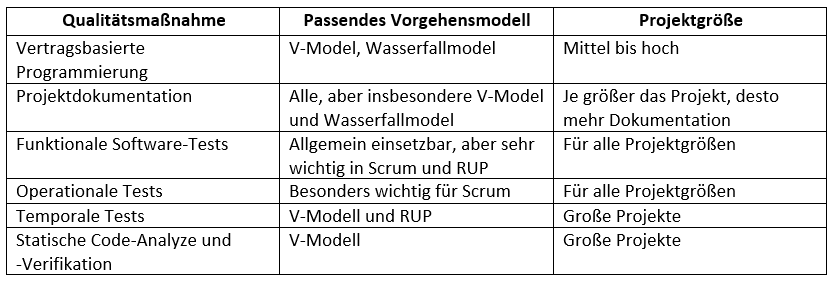
\includegraphics[width=\textwidth, height=\textheight,keepaspectratio]{QualityMassnahmen.png} 
    \caption{Anwendung verschiedener Qualitätsmaßnahmen}
    \label{fig:quality_sicherheit}
\end{figure}
Wie man sieht, werden viele Maßnahmen im V-Modell und nicht in Scrum verwendet, weil im V-Modell der Fokus auf die Qualitätssicherung und Dokumentation gelegt wird. Im Gegensatz dazu wird bei Scrum schneller auf die Anforderungsänderungen reagiert
und es wird schneller ein Ergebnis an den Kunden geliefert. 